%!TEX root = main.tex
% UTF-8 encoding

\newpage
\appendix

\begin{table*}
	\centering
	\caption{Euphemism detection results by our approach (better viewed in color). 
		Purple bold words are correctly detected euphemisms and on the ground truth list (\ie, the DEA list). 
		The purple underlined words indicate that they are incorrect by themselves, but are contained in true euphemism phrases, such as ``dog food", ``Chinese Tobacco" (euphemisms for ``heroin" and ``opium" respectively). 
		Those words which do not appear in the ground truth list are marked black. 
		}
	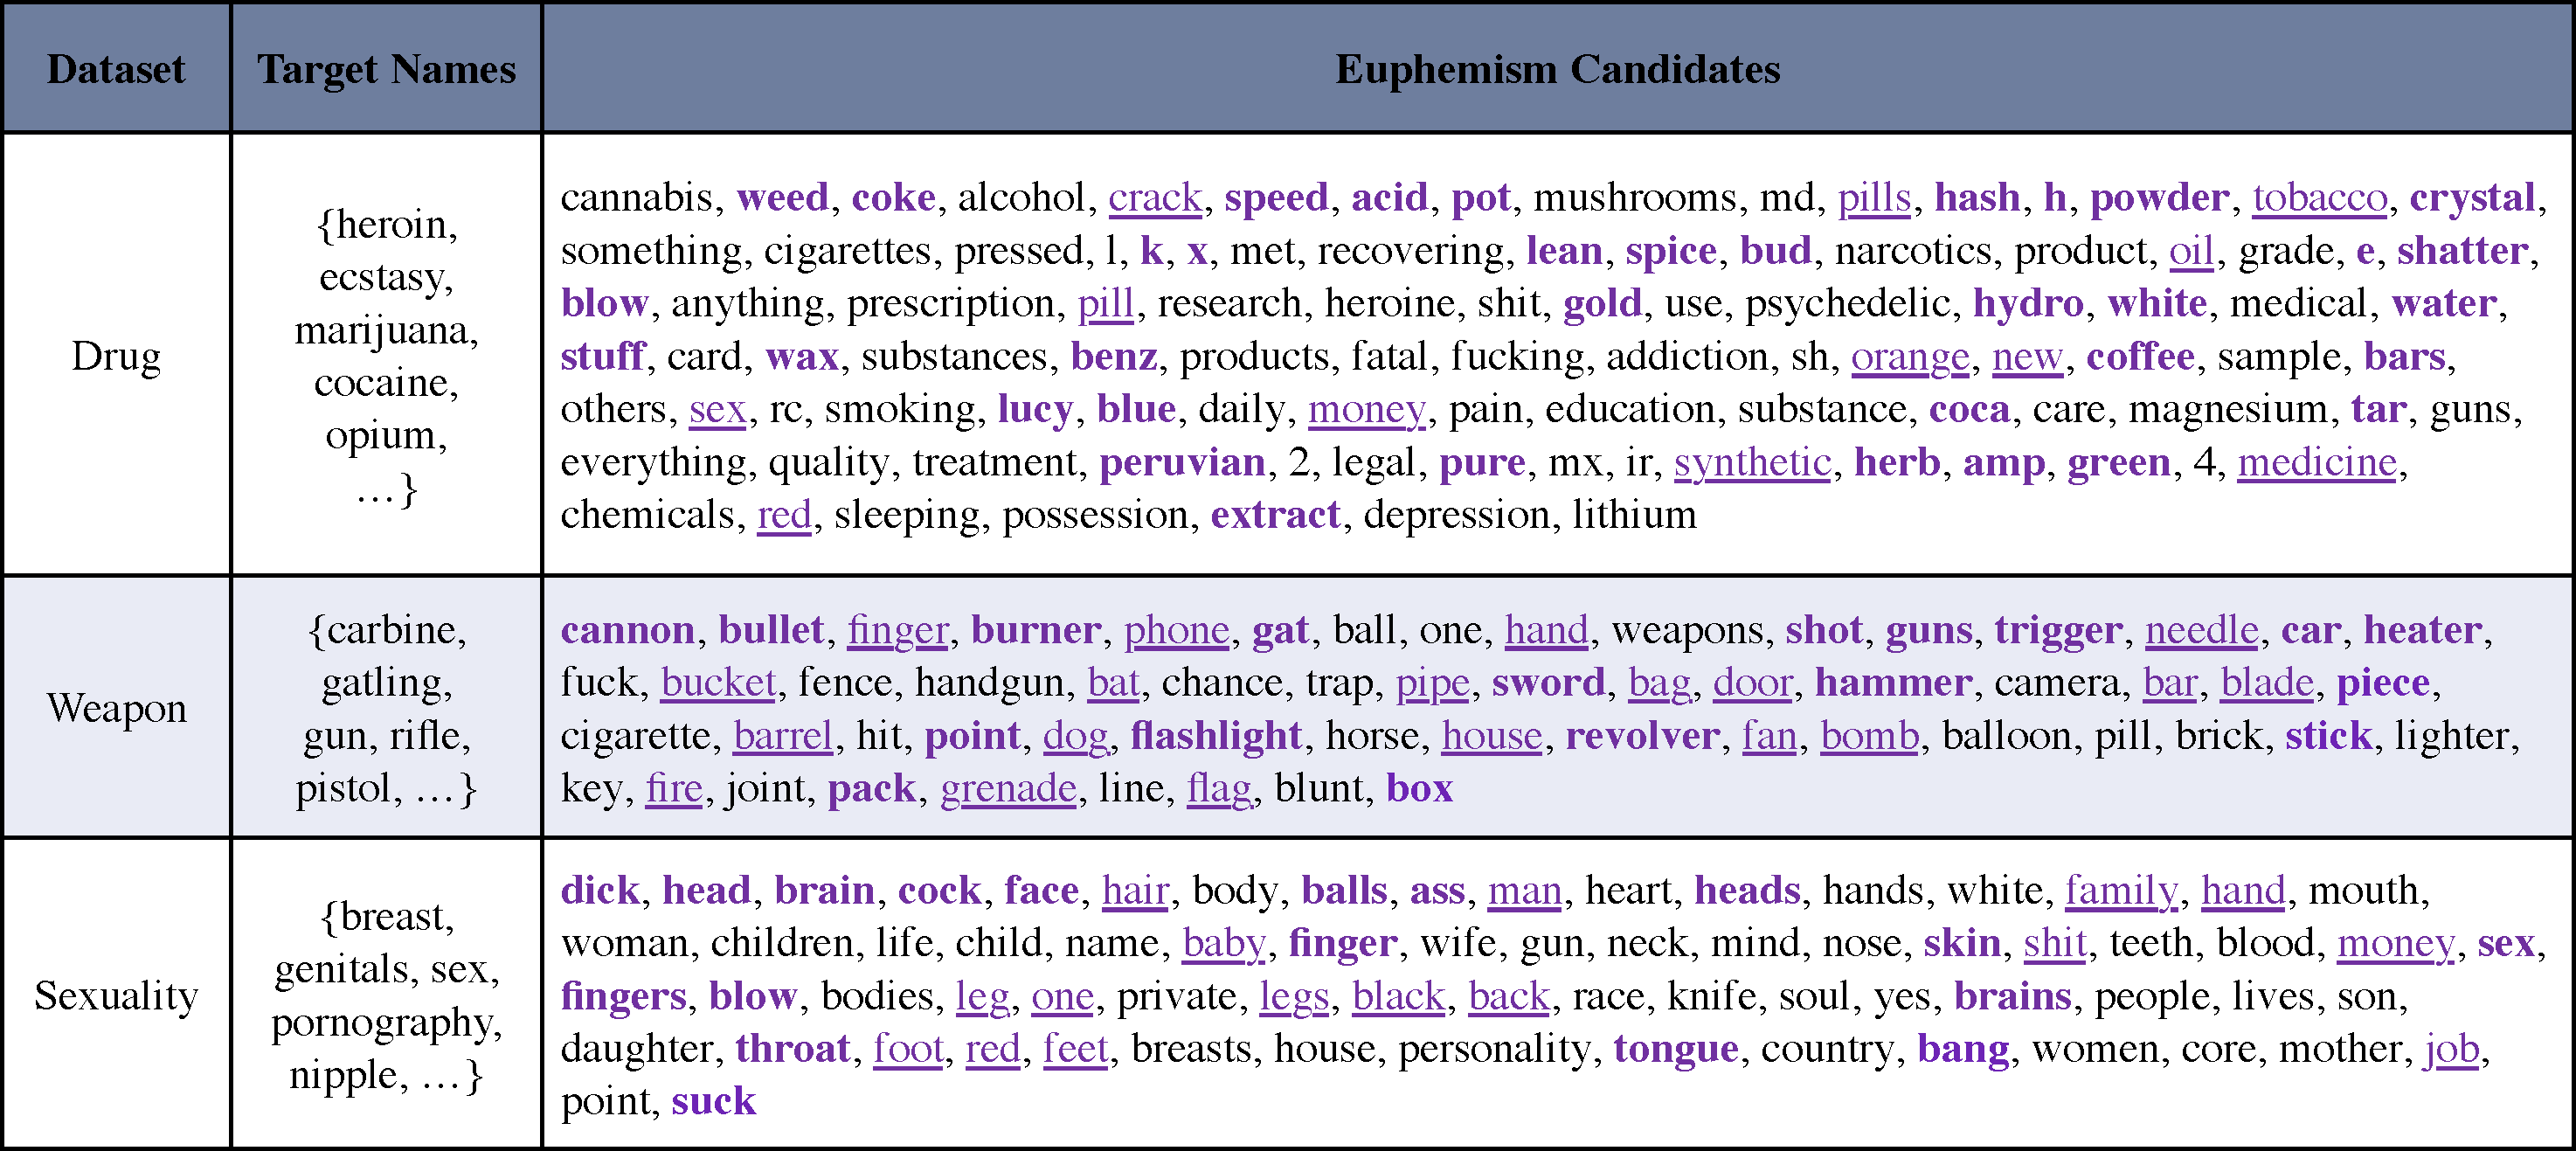
\includegraphics[width=1\linewidth]{figures/CaseStudies-Detection}
	\label{fig:casestudies-detection}
\end{table*}

\begin{table*}
	\centering
	\caption{Case studies of the false positive detection results on the drug dataset. They are real examples from Reddit.}
	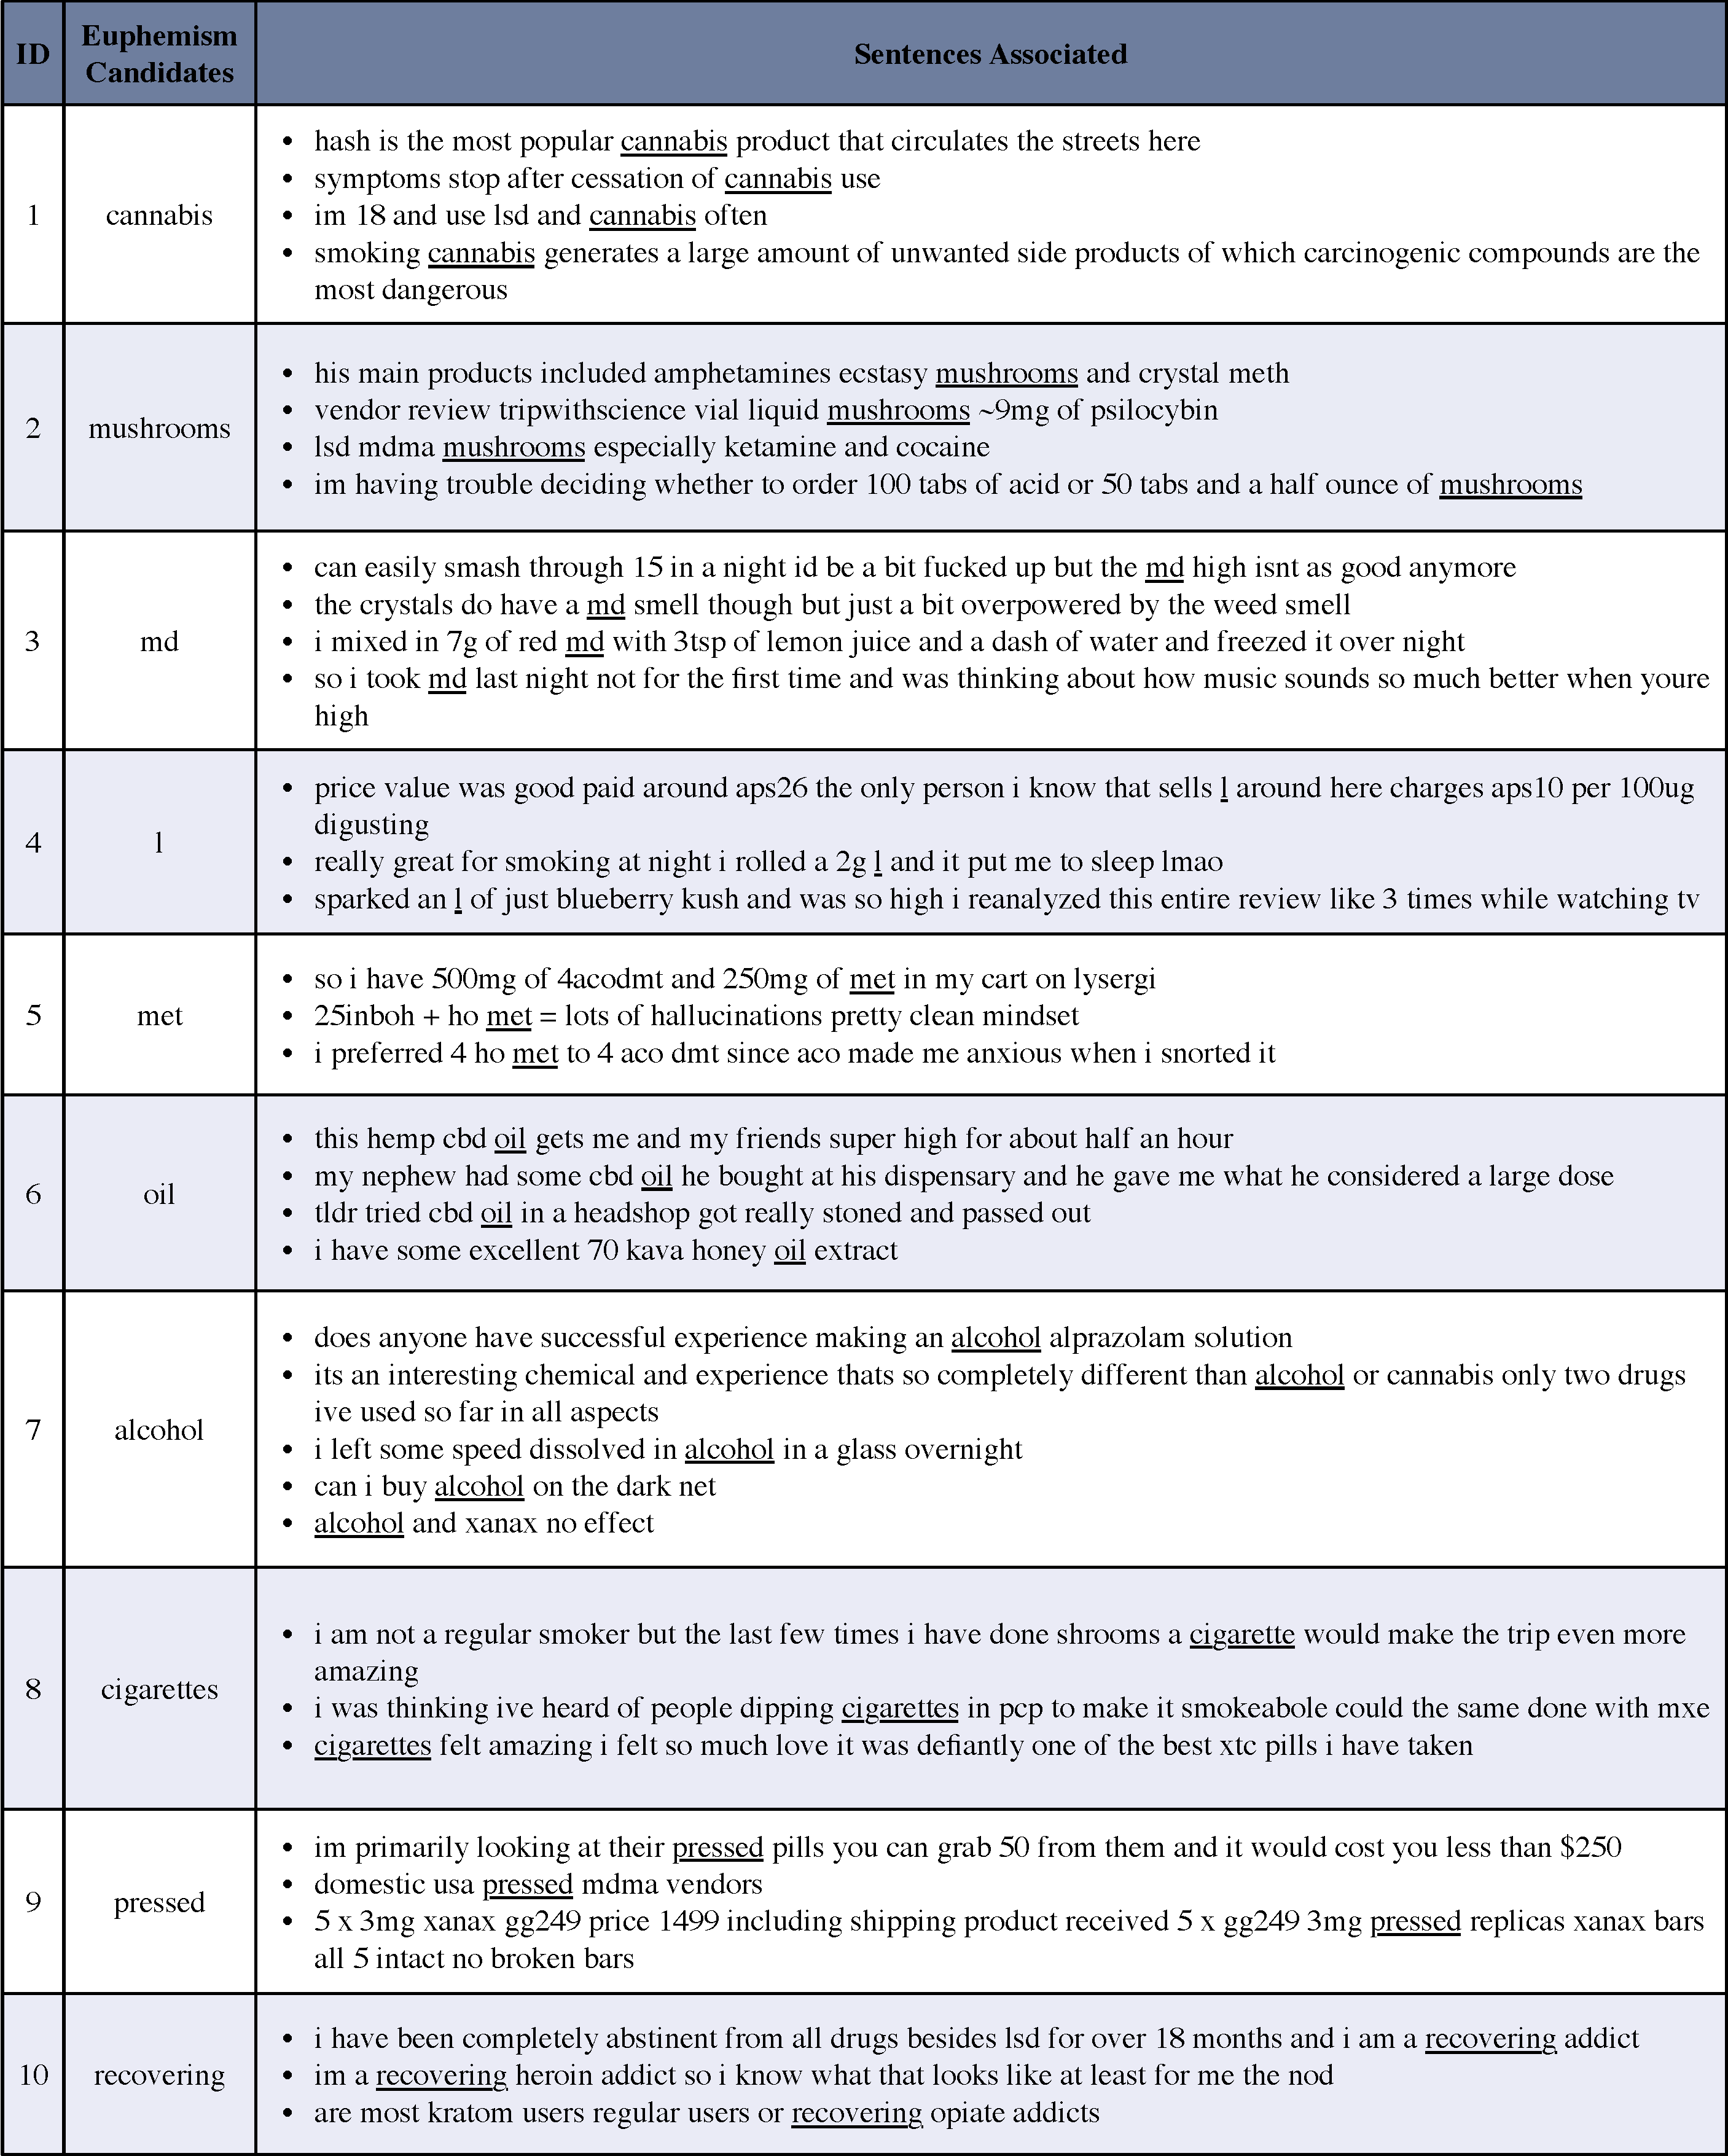
\includegraphics[width=0.96\linewidth]{figures/CaseStudies-Detection2}
	\label{fig:casestudies-detection2}
\end{table*}

\section{Case Study of Euphemism Detection}
\label{sec:appendix}

We present the euphemism detection results by our approach in Table \ref{fig:casestudies-detection} and analyze the false positive detection results on the drug dataset in Table \ref{fig:casestudies-detection2}. 
We categorize our false detection results into four types: 
\begin{itemize}
	\item They are correct euphemisms but missed on the ground truth list (cases 1-5 in Table \ref{fig:casestudies-detection2}). 
	\item They are not euphemisms by themselves, but they are contained in euphemism phrases. For example, as shown in case 6 in Table \ref{fig:casestudies-detection2}, ``oil'' is not a drug euphemism while ``cbd oil'' is one. 
	\item Though they are not euphemisms, they are strongly related to drug or the usage of drug (cases 7-10 in Table \ref{fig:casestudies-detection2}). Cases 7 and 8 uncovers some ways that people take drugs (together with alcohol or cigarettes).
	\item Incorrect detection. 
\end{itemize}

The case studies reveal that we can even find some correct euphemisms that are not on the ground truth list, which suggests the rapid-evolving nature of euphemisms and the necessity of the automatic euphemism detection task. 
